\documentclass[12pt]{article}
\usepackage[utf8]{inputenc}
\usepackage{fullpage}
\usepackage{amssymb}
\usepackage{multicol}
\usepackage{graphicx}
\usepackage{tikz}

%\usepackage{pgffor}   % for 'for loop' usage

%\usepackage{pstricks}

\newcommand{\exerc}[3]{ \vspace*{25pt} {$\mathbf{#1)}$} #2 \hfill {\it #3} }
\newcommand{\exitem}[2]{ \texttt{\bf #1)} #2 \\ }
\newcommand*\xor{\mathbin{\oplus}}

%\newcommand{\clock}[1]{
%    \psset{yunit=0.8}
%	\rput(0,0.1){
%      \foreach \n in {0,...,#1}{
%	  \translate(2,0)
%      \psline
%	    (0,0)(1,0)(1,1)(2,1)
%	  }
%	}
%    \psset{yunit=1.0}
%}

%\newcommand{\signalBlock}[1]{
%  \vspace*{20pt}
%  \hspace*{-30pt}
%  \pscustom[xunit=0.5]{
%    \rput(1,2){#1}
%  }
%}

%\newcommand{\signal}[1]{
%    \psset{yunit=0.8}
%	\rput(0,0.1){
%    \psline
%	  #1
%	  }
%    \psset{yunit=1.0}
%}

\renewcommand{\neg}[1]{ 
  \mkern 1.5mu\overline{\mkern-1.5mu#1\mkern-1.5mu}\mkern 1.5mu
}

\newenvironment{exitems}[1]{
\\
\hspace*{30pt}
\begin{minipage}{0.8\textwidth}
\begin{multicols}{#1} 
}{
\end{multicols}
\end{minipage}
}

\newenvironment{exitemss}[1]{
\\
\hspace*{30pt}
\begin{minipage}{0.8\textwidth}
#1
}{
\end{minipage}
}

\newcommand*\circled[1]{\tikz[baseline=(char.base)]{
            \node[shape=circle,draw,inner sep=2pt] (char) {#1};}}

\begin{document}

\pagenumbering{gobble}

\begin{center}
{\Large \bf Elementos de Lógica Digital - 2015/2}
\end{center}

{\large \bf Lista de exercícios}

{\bf Professor:} Marcos Daniel Baroni

{\bf Data:} 29/10/2015


\exerc{1}{Esquematize um contador assíncrono que conte de $0$ a $15$ e possua uma entrada 'X'
	que ao ser acionada faz com que a contagem seja feita em ordem decrescente.}{}

\exerc{2}{Esquematize um contador síncrono que conte a sequencia
	$\circled{0} \rightarrow
	\circled{5} \rightarrow
	\circled{2} \rightarrow
	\circled{7} \rightarrow
	\circled{3} \rightarrow
	\circled{6} \rightarrow
	\circled{1} \rightarrow \circled{5}$ e possua uma entrada 'X' que ao ser acionada faz com que a contagem
 	seja feita em ordem reversa.}{}

\exerc{3}{O contador abaixo realiza a contagem de qual sequencia?}{}
\begin{center}
		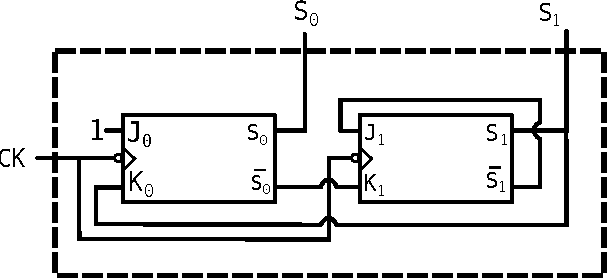
\includegraphics[scale=0.6]{cont1} \\ \vspace{15pt}
\end{center}

\exerc{4}{ A partir de dois blocos demultiplex de 16 canais e um de 2 canais, forme um sistema demultiplex de 32 canais.}{}

\exerc{5}{ Esquematize o circuito interno de um multiplexador de 16 canais.}{}

\exerc{6}{ Utilizando células básicas de memória, esquematize o circuito interno de uma RAM (a) 8x4 e (b) 4x8.}{}


\exerc{7}{Defina
(I) capacidade total de memória (em bits),
(II) largura de palavra de dados,
(III) largura da barra de endereços e
(IV) palavra de endereço final
para as seguintes memórias:}{}
\begin{exitems}{2}
	\exitem{a}{ 16k x 8 }
	\exitem{b}{ 64 x 4 }
	\exitem{c}{ 1M x 16 }
	\\
	\exitem{d}{ 128 x 8 }
	\exitem{e}{ 64K x 8 }
	\exitem{f}{ 2M x 16 }
\end{exitems}

%\exerc{8a}{A partir de blocos RAM 64x4, esquematize uma RAM 64x8.
%Escreva as palavras de endereçamento inicial e final de cada RAM integrada
%ao sistema.}{}
%\exerc{8b}{Idem ao item anterior, para obter uma RAM 512x4 com blocos de estrutura 128x4.}{}

%\exerc{8c}{Idem, para obter uma RAM 64x8, obtidas com blocos de estrutura 32x4.}{}
\end{document}

